% Please use the skeleton file you have received in the 
% invitation-to-submit email, where your data are already
% filled in. Otherwise please make sure you insert your 
% data according to the instructions in PoSauthmanual.pdf
\documentclass{PoS}

\title{Data transfer infrastructure for CMS data taking}

\ShortTitle{Data transfer infrastructure for CMS data taking}

\author{
  \speaker{Ricky Egeland},$^a$ Tony Wildish,$^{b}$ and Simon Metson$^{c}$\\ 
  \llap{$^a$}University of Minnesota, Twin Cities\\ 
  \llap{$^b$}Princeton University\\ 
  \llap{$^c$}Bristol University\\ 
  E-mail: \email{Ricky.Egeland@cern.ch}, \email{Tony.Wildish@cern.ch}, \email{Simon.Metson@cern.ch}
} 

\abstract{The CMS PhEDEx (Physics Experiment Data Export) project is
responsible for facilitating large-scale data transfers across the
grid ensuring transfer reliability, enforcing data placement policy,
and accurately reporting results and performance statistics. The
system has evolved considerably since its creation in 2004, and has
been used daily by CMS since then. Currently CMS tracks over 2 PB of
data in PhEDEx, and it has been tested well beyond the requirements of
CMS. Over the past year PhEDEx has evolved considerably, making use of
new technologies (chiefly POE, an asynchronous, event-driven,
cooperative-multitasking framework) and to consolidate the various
components such that it is easy to reuse existing techniques and
components in new features. This has resulted in changes to nearly
every piece of the PhEDEx code base, creating a flexible modular
framework. We are able to evolve the implementation to match changes
in the requirements of the experiment, without changing the
fundamental design. Two major new features have recently been added to
the PhEDEx system; an extensible data service and an improved transfer
back-end module. The extensible data service provides machine-readable
data over HTTP as the primary means of integration with other CMS
services. An authenticated command line interface is also provided,
making it possible to provide new utilities quickly with minimal
development effort. The new transfer back-end module now integrates
closely with FTS, the glite provided transfer tool, to provide
accurate status information while keeping as much data in flight as
possible. The new transfer back-end is transfer technology
independent, and we expect to be able to support new transfer tools as
they become available. We describe the CMS PhEDEx system that is in
place for CMS ``first data taking'' in 2008, provide details on the
benefits and implementations of the new features, and describe other
new tools that are now available.}

\FullConference{XII Advanced Computing and Analysis Techniques in Physics Research\\
		 November 3-7 2008\\
		 Erice, Italy}

\begin{document}

\section{Introduction}

In order to meet the data distribution requirements
\cite{cms-comp-proposal, cms-comp-tdr, cms-comp-model} of the CMS
\cite{cms-proposal} experiment at the LHC, the Physics Experiment Data
Export (PhEDEx) \cite{phedex-chep06, phedex-chep07} project was
designed to facilitate and manage global data transfers over the grid.
Since its conception in 2004, it evolved considerably until version
2.5 was released in early 2007 and has been shown to be a robust,
reliable, and scalable system which has guided over 62 million
transfers and over 67 PB of data.  PhEDEx provides a simple mechanism
to request the transfer of thousands of files at a time, which then
sets into motion an array of special-purpose software ``agents''
progressing the transfer state machine to the desired end --- files on
disk at the destination.  Reliability is ensured by independently
verifying each file transfer when it lands at the destination,
robustness is achieved by intelligently backing off when large numbers
of failures are encountered.  Through numerous challenges and daily
use for months, the transfer management layer of PhEDEx is not in
question.

More recent developments have focused on improving the ease of
development, the ease of use, and integration of PhEDEx with grid
infrastructure such as FTS and SRMv2 as well as with other CMS data
management components.  These developments did not require extensive
redesign of the business logic of core PhEDEx components such as the
file router and the site download agents.  PhEDEx has adopted the Perl
Object Environment (POE) as its scheduling and event manager for the
agents.  The agents have been modularized into separate libraries for
SQL and business logic, for greater reusability of SQL and simplified
debugging.  For integration with FTS, a new transfer backend was
developed.  For integration with other data management components, a
web data service for providing XML or JSON via HTTP requests was
developed using Apache and mod\_perl.  Finally, a framework was
developed for performing consistency checks to compare database and
disk consistency in a controlled fashion.  These recent developments
are the focus of this paper, following an overview of the
project and performance acheivements.

\section{Overview of CMS Computing and PhEDEx}

CMS uses the combined resources of over 60 data centers around the
world providing over 5 PB of storage space.  They are divided into
four tiers defined by their service requirements to the experiment.
At the host of the experiment, CERN, the Tier 0 is the origin of
experiment raw data and the products of first processing.  The role of
PhEDEx in the Tier 0 is to replicate these irreplaceable data to the
various tier 1 centers before the buffers at the Tier 0 become full.
CMS must reliably export data at an average rate of 625 MB/s to the tier 1
centers in order to keep up with data production.  The tier 1 centers
have a custodial responsibility for safekeeping the Tier 0 data as
well as performing processing in order to provide more useful
data products for analysis at the Tier 2 centers.  The tier 2 centers,
of which there are over 50, are dedicated to two purposes: to serve as
analysis centers for physicists and producing monte carlo data.
Analysis products must be transferred to the tier 2 from the tier 1
and tier 2 produced monte carlo data must be transferred to the tier 1
for custodial storage.  Finally there are the tier 3 centers which are
smaller sites that typically are only interested in receiving data for
analysis and have no specific storage or processing responsibilities within CMS.

PhEDEx manages transfers using a high-availability Oracle database
cluster hosted at CERN as a ``blackboard'' for the system state.  This
database is known as the Transfer Management Data Base, or TMDB.
Software daemon processes or ``agents'' connect directly to the
database to query for the current state and perform the actions
necessary to bring the system to the desired state, which is then
written back to TMDB.  Central agents running at CERN perform most of
the intelligence of data routing and transfer task creation.  The
download agents running at the site receive these tasks and initiate
the data transfers using a technology-specific backend interacting
with the grid middleware.  After a transfer attempt, the file is
verified using a site-specific script, and it is the result of that
verification which is used to indicate success or failure of the
transfer, not any specific return code or message from the grid tools.
PhEDEx is a level-triggered as opposed to an edge-triggered system in
that it builds large work queues which are largely unaffected by state
changes in the steps preceding until the next work cycle.  This allows
the system to have self-healing properties and avoid widespread damage
from isolated errors or transient bugs in a work cycle.  The TMDB has
been carefully designed to minimize locking contention between the
several agents and cache coherency issues by using an row
``ownership'' model where only one piece of software at a time is
expected to act on a given set of rows.

\begin{figure}[htp] 
\centering
\setlength\fboxsep{0pt} 
\setlength\fboxrule{0.5pt} 
\fbox{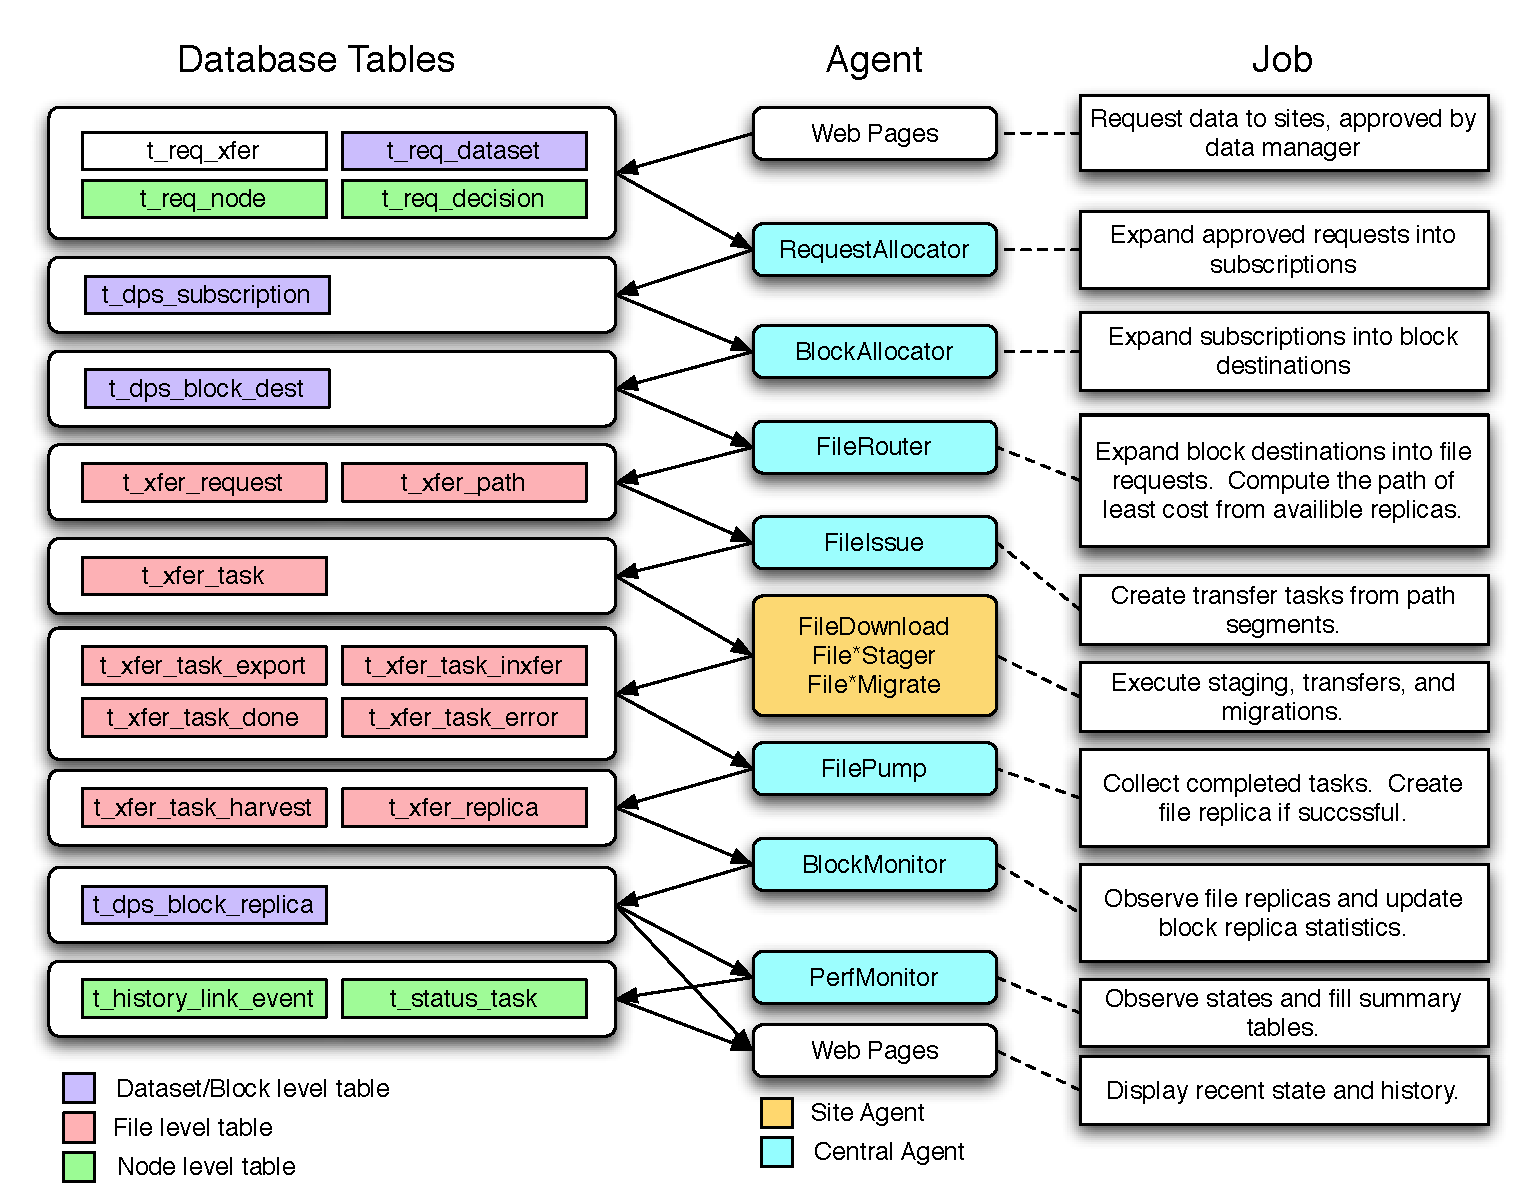
\includegraphics[width=.8\textwidth]{workflow.pdf}}
\caption{PhEDEx transfer workflow, the relationship between agents and the schema}
\label{fig:workflow}
\end{figure}

Users of PhEDEx interact with the system via a web interface which
provides administration functions as well as monitoring information.
Users are typically CMS operations staff or site administrators,
although some physicists interact with the system to subscribe data to
their assigned tier 2 center.  Users make transfer requests via a
simple web form where they indicate the destination nodes and the
datasets they wish to transfer.  Data managers assigned to each site
receive a notification email and make the decision whether to approve
or refuse the request.  Approved requests become subscriptions, which
are then handled by the workflow, routing, and finally the site
download agents to result in files on the disk at the desired node.
Requests for deletion of data at the node are handled in a similar
manner, although the workflow is more straightforward as it only
involves work for a single node.

Monitoring information is available from the website which represents
a recent, but not current state of TMDB.  Load on the database is
reduced by summarizing monitoring information into special purpose
status tables at regular intervals.  By building monitoring tools
based on these tables instead of those with the current state,
response times are reduced and the user experience is improved.
Historical information is regularly aggregated from these status
tables into variable-width bins of data on transfer volume, transfer
state counts, and number of failures.  The monitoring itself
introduces little load on the system and the time to access is a
function of the time span the user is interested in and is not
affected by the current load of the transfer system itself.

\section{Performance and Release Preparation}

PhEDEx 3.0 was extensively tested before release on a dedicated
validation cluster in order to ensure no performance issues were
introduced by the changes.  Two different types of validation runs
were performed: a router scaling test which was designed to stress the
database and core components to the maximum level possible, and a
``data lifecycle'' simulation which was designed to exercise all
components of the system in a more realistic workflow.

The router scaling test starts from an initial state of 100,000 files
evenly distributed across 8 tier 1 and 50 tier 2 nodes, for a total of
66 nodes (tier 1 sites are represented as two nodes, a ``Buffer'' for
outgoing/incoming transfers and the ``MSS'' (Mass Storage System)
which represents tape storage).  Each node is then subscribed to all
the available data, making the final state 6.6 million replicas.  The
central agents ran on a dedicated box we had direct access to, so we
could monitor the progress of the test.  The site agents were run as
batch jobs to the computing cluster with each download agent running
for up to five nodes simultaneously.  No actual file transfers were
performed, instead a successful transfer was immediately reported at
the point where the transfer would be initiated.  The test ran for a
total of 10 hours and achieved a replica creation rate of nearly 1
million files per hour for the first 6 hours.  The last 4 hours were
limited by the test configuration of the tier 1 nodes which prevented
them from transferring between them in parallel.  If corrected, it is
expected that the tier 1 nodes would transfer at the same rate as the
tier 2 nodes, and the 4 hour tail would be eliminated.  The fictional
replication rate achieved in this setup far exceeds the requirements
of CMS, and proved that our transfer system will be limited by
bandwidth and site storage issues, not the transfer management system..

\begin{figure}[htp] 
\centering
\setlength\fboxsep{0pt} 
\setlength\fboxrule{0.5pt} 
\fbox{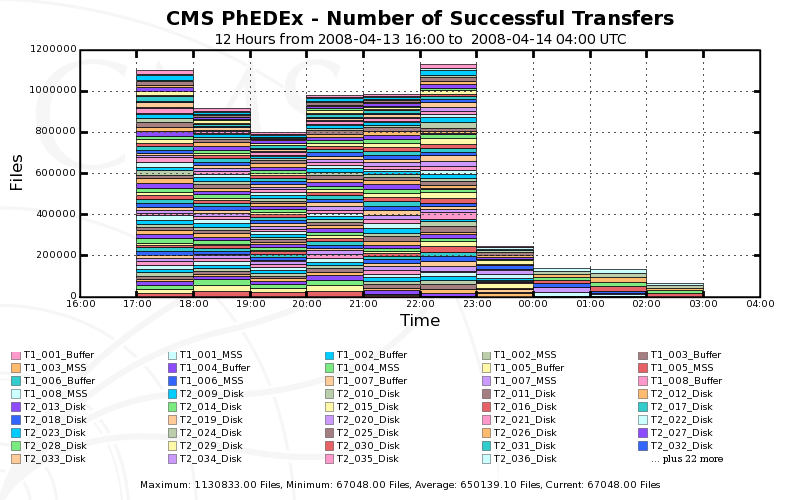
\includegraphics[width=.8\textwidth]{phedex-scaling08-success.png}}
\caption{PhEDEx 3.0 scaling test results --- number of successful transfers per hour}
\label{fig:scaling08}
\end{figure} 

The lifecycle test is another no-transfer test that exercises more of
the PhEDEx code base than the router scaling test and is designed to
run for an extended period of time.  In this test, the initial state
is an empty database, and the ``lifecycle agent'' simulates the
plausible behavior of other CMS components and users.  The lifecycle
agent regularly injects new file replicas at various nodes at various
sizes and frequencies, simulating data production as expected in CMS
running.  Subscriptions are then made to other nodes and data is
transferred.  Some of the data is then marked for deletion, simulating
that part of the workflow.  Furthermore, each of the node-to-node
links had a configurable probability for transfer failure, allowing us
to exercise error handling and retry operations.  The entire simulated
computing model is dynamically configurable allowing us to test a
range of usage patterns.  A single scaling factor allowed us to run
this simulation at some factor greater than the expected reality.
This test ran for two full days and by the end managed 6.5 million
files and achieved 14 million replicas.  Due to various time
constraints we were not able to run this test as cleanly as we would
like and fully investigate the results, but the preliminary conclusion
was that the system would continue to run well whilst tracking over 2
times more files and replicas than we expected to have in 2009 and at
100x the expected activity rates.  The lifecycle agent itself is
capable of running even more simulated actions on the system.  In
future tests we also intend to simulate website and data service
usage.

In parallel to the performance validation and scale testing, volunteer
site administrators participated in real-world tests of pre-release
RPMs of PhEDEx 3.0 using our infinite transfer LoadTest framework.
Feedback from these tests gave us fast feedback on oversights and
omissions of the release, particularly with respect to the new FTS
backend.  Fixes were made for the most important concern, resulting in
a release which we were confident could be widely adopted with little
disturbance to ongoing activities.

We cannot stress enough the importance of this kind of multi-faceted
testing for a major release of distributed computing software.
Releasing without absolute confidence in the performance, scalability,
and a usable feature set would only result in chaos and many lost
man-hours for system recovery.

\section{CCRC'08 Achievements}

PhEDEx 3.0 was released as a mandatory upgrade less than two weeks
before the WLCG CCRC'08 phase 2 \cite{ccrc08}, the most significant computing
challenge CMS had participated in up to that point.  During CCRC'08,
PhEDEx managed the successful transfer of an average of 120 TB per day
for 29 days over hundreds of site links, for a total of over 3.6 PB of
data transferred.  44\% of these transfers were on the production
instance, composed of monte-carlo data and with tier 1 tape systems in
use.  The remaining 56\% was on our ``debug'' LoadTest instance \cite{ddt-final}, which
creates new transfers from small source samples and does not involve
tape systems or permanent data storage.

CCRC'08 was designed to stress the grid systems at a significant
fraction of expected start-up levels.  CMS set transfer targets for
each of the tier 1 sites from the Tier 0 and among its regional tier 2
sites.  Nearly all of the transfer targets were met and the transfer
infrastructure was considered ready for the expected start up volumes
of fall 2008.

\begin{figure}[htp] 
\centering
\setlength\fboxsep{0pt} 
\setlength\fboxrule{0.5pt} 
\fbox{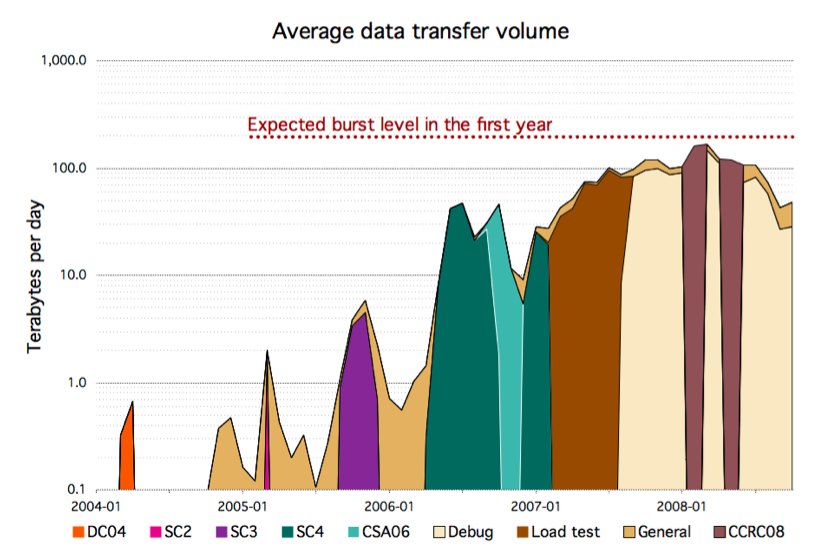
\includegraphics[width=.8\textwidth]{phedex-daily-volume.png}}
\caption{Daily transfer volume using PhEDEx since its creation.
Highlighted are the various data challenges, the most recent being
CCRC'08/phase 2 which acheived rates of 120 TB/day.}
\label{fig:daily-volume}
\end{figure}

\section{Data Service}

In order to better integrate with other CMS data and workflow
management components, a web data service was developed for PhEDEx.
This service is the first public API for exchanging information with
the system.  The data service provides data in XML, JSON, or perl
objects to clients passing API calls and parameters in the request
URL.  The three data formats are automatically generated from perl
objects returned by the web API backend modules.  Only authorized
users registered in CMS SiteDB with the appropriate role/group for the
specific action are allowed.  This web service was implemented in
Apache/mod\_perl and is deployed on a 3 node cluster running in a
reverse proxy configuration with a secure frontend for grid
certificate authentication.

Currently, the data service provides APIs for data location, file name
translations, data injection, and subscribing data.  These functions
are being integrated with CMS production systems in order to easily
automate workflows which require data transfers.  Extending the data
service is as simple as adding a new perl module to the appropriate
namespace, enabling rapid prototyping and deployment.  A command-line
interface is also provided to interact with the data service for both
read and write operations.  Soon after the release of the data service
industrious site administrators in the CMS community began developing
custom applications which make use of it for their monitoring.  We
hope to see this trend continue.  Finally, the data service is planned
to become the primary data source of a future AJAX-based website.

\section{Use of POE}

POE \cite{poe} is the 'Perl Object Environment', a framework for creating
event-driven cooperative multitasking programs in Perl. POE threads,
or 'sessions', communicate via event-messages with arbitrarily
customisable payloads. POE is 10 years old and under active
development. It provides several components at all levels of
abstraction that make the construction of complex programs very easy.

Cooperative multitasking in the same process makes the interfaces
between components lightweight, easy to develop and debug, and
performant. Components can be developed standalone and then plugged
into the same process with little effort. For example, a component
which monitors the value of some external resource and provides a
method to return the result can be developed in isolation and then
directly dropped into the program. The traditional problems of race
conditions in multi-threaded environments simply do not occur. On the
other hand, a single component locking up can block the entire
process, so care must be taken to ensure this does not happen. It is
intrisically easier to prevent intra-component lockup than
inter-component race conditions, and POE has good support for handling
this problem.  Database-oriented tasks such as those embodied in
PhEDEx are well suited to this type of programming, as
transaction-oriented code can be embodied in single event-handlers,
running without interruption from other threads.

Use of POE makes it possible to run multiple PhEDEx agents in one
process, something that was not possible before. Agents which would in
the past have contended for resources on the database can now be
managed as cooperative threads, even sharing a database
connection. This lowers load and connectivity on the database, and
avoids wasted context switches and excessive process load.

\section{The FTS backend}

The core data-movement engines of PhEDEx are the ``backend'' modules to
the FileDownload agent. One of these is the FTS backend, which is
responsible for submitting transfer jobs to the grid File Transfer
Service (FTS) \cite{fts}, monitoring the transfers, and acting on the
success or failure of the individual transfers. A significant feature
of PhEDEx 3.0 and its further development through 2008 has been the
redesign of the FTS backend to achieve better throughput and reporting
with lower load on both the PhEDEx service and the FTS service.

Before PhEDEx 3.0, the FTS backend would prepare a transfer job to
submit to the FTS service, submit it, and then wait for the job to complete
before examining and acting on the results. A separate subprocess
would monitor each transfer job, one subprocess per job, and only when
the job ended would that subprocess be harvested by the FTS backend to
get the results. A single stuck file would therefore cause knowledge
of the state of all the files in the job to be delayed, with the
consequence that available transfer slots might be left idle
unwittingly. In order to promote efficient use of the netowrk, sites
often configured their FileDownload agents to transfer only one file
per FTS transfer job. This meant that an excessive number of
transfer jobs were submitted to the FTS service, and that large
numbers of transfer monitoring processes could place a heavy load on
the machine. Since the transfer monitoring processes were
independent, they could also place an unreasonable burden on the FTS
service, polling it at a rate which was directly proportional to the
number of submitted transfer jobs.

In order to fine-tune bandwidth used per link, sites often configured
one FileDownload agent per transfer link, instead of allowing one
agent to handle many links. This meant that sites were running many
more FileDownload agents than necessary, which translated into many
unnecessary connections to the central PhEDEx database. It also meant
that the FileDownload agent was deprived of the opportunity to
optimise throughput by choosing among links when preparing to submit
transfer jobs.

For PhEDEx 3.0 the FTS backend was refactored significantly. FTS
transfers are now performed by three interacting components, the
remodelled FTS backend, the Queue Monitor, and the Glite interface.

\begin{figure}[htp] 
\centering
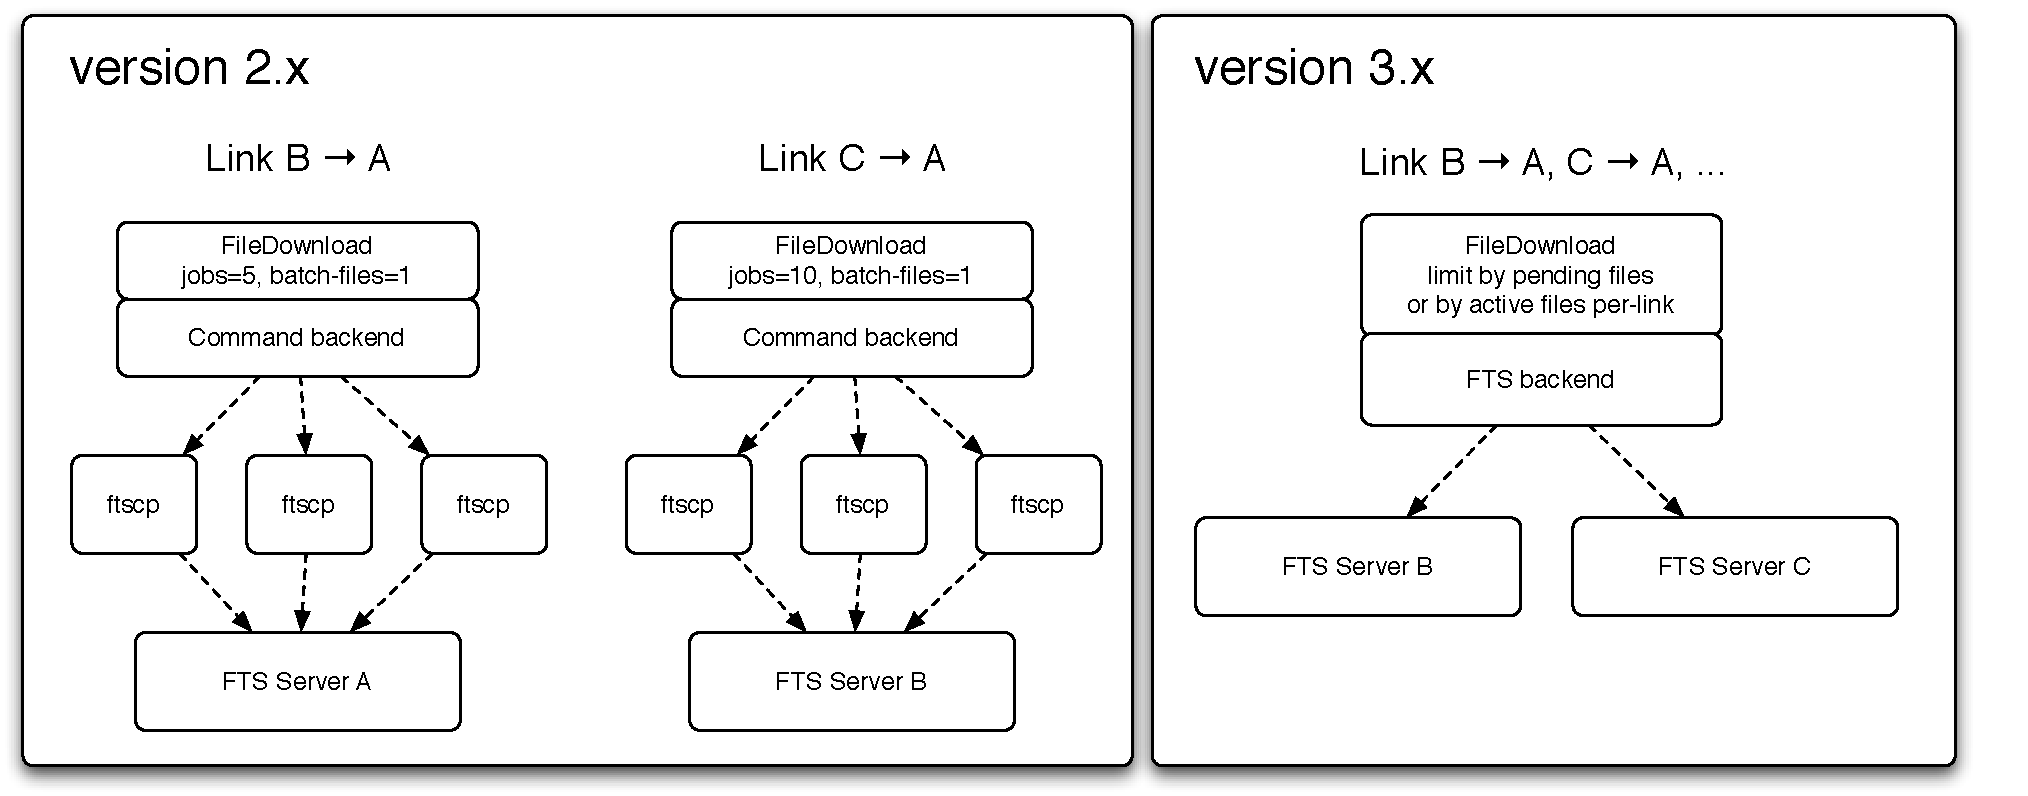
\includegraphics[width=.8\textwidth]{fts-combined.pdf}
\caption{FTS backend in PhEDEx, before and after PhEDEx 3.0}
\label{fig:fts}
\end{figure} 

The FTS backend itself takes care of parceling the file queue into
discrete chunks that are submitted as FTS transfer jobs, and of
harvesting the results and uploading the status to the PhEDEx
database. It uses the Glite component to perform the actual
submission, decoupling it from the details of the command syntax. The
FTS backend also uses the Queue Monitor to determine the state of the
jobs that are submitted. It simply notifies the Queue Monitor that a
job has been submitted, and lets the Queue Monitor take care of it
from then on.

The Queue Monitor maintains a list of transfer jobs that it knows
about and periodically checks the status of jobs. It uses the Glite
component to execute the monitoring command and return the result. The
Queue Monitor checks jobs in a round-robin manner with a fixed
interval between checks, so places a constant load on the FTS service
regardless of the number of jobs submitted. The POE 'postback'
mechanism (essentially asynchronous callbacks) allows the monitor to
notify the FTS backend of the change of state of each file in a
transfer job independantly, so the FTS backend can act on completed
file transfers (successful or otherwise) while the rest of the files
in a transfer job are still in transit.

The Queue Monitor also maintains details of file state and link state
for all the files and transfer links it is monitoring. This
information is used by the FTS backend to throttle transfers and to
select among links. The information is updated perodically, as each
job is monitored, so is not real time, but it does not need to be. The
fact that file-state information is available while the transfer job
is still executing is enough to make the system adequately performant,
as fewer transfer jobs need to be submitted so the interval for
monitoring a single job is fairly short.

The Glite component is responsible for constructing the commands for
submitting, monitoring, and changing the priority of FTS
transfer jobs. It executes the commands and parses the output,
returning the result to the calling component as a Perl hash. This
encapsulates the interaction with the FTS service completely, nothing
else in the system need know any of the details of the command
syntax. In PhEDEx 3.0.0 the Glite component executed the commands
synchronously, but later releases used POE components (specifically
POE::Component::Child) to execute the commands asynchronously, passing
the results back using the POE postback mechanism. This was necessary
to prevent problems with the glite commands blocking the entire
transfer agent.

\section{The Consistency Tools Project}

There are many levels at which inconsistencies can occur between
storage systems and internal CMS bookkeeping. Simple database
inconsistencies between the transfer service (PhEDEx) and the CMS
Dataset Bookkeeping Service (DBS) can arise under some circumstances,
files can arrive on disk and then fail to migrate to tape, disks and
tapes can fail in many ways, files can become corrupt in copying
between disks, and finally, human error cannot be prevented.

With the ever-increasing number of files shipped by PhEDEx, there is a
corresponding increase in the effort required to detect and recover
from such errors. It is becoming more and more important to have
automated tools to check that data really is where we claim it to
be. The consistency tools aim to bridge that gap.

The PhEDEx Consistency tools are a set of command-line tools and
agents for verifying the consistency of data at a site. They provide a
number of lightweight checks for consistency in a controlled
manner. ``Lightweight'' means they provide namespace checks to verify
that all files of a block or dataset are in the same state, that files
known to PhEDEx are known to DBS and to the underlying Storage
Element, that file sizes are consistent with that recorded in PhEDEx,
and (where relevant) that migration to tape was successful. By
scheduling tests through an agent, instead of running them
immediately, we allow the possibility to test large volumes of data
without placing undue load on the Storage Element, and without users
having to maintain open terminal sessions connected to long-running
scripts. Interactive tools are provided, but are not recommended for
testing large volumes of data.

The tools do not verify checksums of files, because that would be too
resource-intensive. Checksumming all the files at a tier 1 center would be a
major undertaking, even if only those on disk were considered. The
bandwidth and CPU required to checksum even a modest fraction of the
files in a reasonable timescale would be prohibitive. If checksumming
were throttled, so that it took several days or weeks to go through
all the files available, then the information becomes stale. There is
no guarantee that the files that were verified a week ago have not
been lost in the meantime.

In fact this principle pervades the consistency tools design. Any
information about consistency between a database and a storage system
will have a degree of confidence associated with it, which decays with
time. Instead of aiming for the impossible goal of being certain about
the state of all data, the tools provide the means to test the state
of data at a rate which does not impact the Storage Element, and which
can be prioritised to accomodate the most important data first. Rather
than attempt to resolve every possible problem, these tools
specifically target the needs to reduce the time operators spend in
tackling the more frequent problems.

A single BlockConsistency agent is run at each site, configured to
have direct local access to the Storage Element. Remote access via SRM
is supported, but is too slow to be of much practical use. The agent
processes a prioritised queue of requests for a set of PhEDEx nodes
that it supports (e.g the Buffer and MSS nodes of a given site) and
stores the results back in TMDB. The results are available through the
web or by use of a command-line reporting tool. Requests which are
deemed too old, because they were not high enough priority to have
been processed in time, are expired from the queue.

A single central agent, the BlockDownloadVerifyInjector agent, looks
regularly for blocks that are not being transferred in a timely
manner. These can be blocks that are delayed in transfer on the WAN or
on the LAN (between Buffer and MSS nodes). For blocks that are delayed
on the WAN, a test request is scheduled for the source data, checking
the filesizes. This should alert operators to transfers which are
failing repeatedly because of files that are the wrong size or, more
commonly, do not exist at the source for whatever reason. For overdue
LAN transfers, tape migration is checked at the destination, to see if
there are any problems there.

The BlockDownloadVerifyInjector agent also performs various
housecleaning tasks, to prevent excessive growth of the database
tables. This helps to ensure that, no matter what volume of data the
users request to check, the system will not become overloaded.

The consistency tools were not widely deployed or used until the
summer of 2008. Following the first round of feedback, there are ideas
for their future development. The most interesting direction is to
allow external components to inject tests and examine results
programmatically, so that tests can be more readily automated in
response to problems detected in other areas of the CMS workflow. For
example, a user's analysis job running at a site may encounter errors,
which could lead to the automatic verification of the data the user
was accessing. Another possibility is to monitor the access to data,
by users or other swcheduled activity, and to pre-emptively verify the
state of associated data, in different data tiers perhaps. The
agent-based verification and associated command-line tools provide a
sound basis for such further development with little or no risk of
impacting more important parts of the system.

\section{Conclusion}

PhEDEx has a long history of transfer management for CMS, and has
reliably managed the transfer of petabytes of data.  In simulation it
has proven its capability for the task well beyond the requirements.
In practice it has reliably met the needs of daily grid computing
activity and the benchmarks of data challenges.  The transfer system
is stable over long time scales, and has sustained transfer rates at
near the expected \emph{burst levels} of running at LHC start-up for
\emph{months}.  Most of the remaining problems with large scale data
transfers fall below the layer which PhEDEx occupies, meaning site
storage systems and grid transfer tools.  Further development of
PhEDEx is focused on providing more information for detecting and
addressing problems early, as well as improving integration with other
components and ease of use.  The PhEDEx software platform is ready to
meet the challenges of the LHC data-taking era.

\bibliographystyle{unsrt}
\bibliography{phedex-acat08}

\end{document}
